\section{Data Encoding with Triplet Network}

Our proposed semi-supervised classification approach addresses another critical challenge in clustering, particularly when dealing with high-dimensional data, by combining Contrastive Learning techniques \cite{Hoffer_2015,Khosla_2020} with Stochastic Quantization. While the Stochastic Quantization algorithm (\ref{sq-objective-fn-gradient:eq}) effectively resolves the scalability issue for large datasets, it, like other clustering methods relying on distance minimization (e.g., K-Means and K-Means++), is susceptible to the "curse of dimensionality". Kriegel et al. \cite{Kriegel_Kröger_Zimek_2009} elucidated this phenomenon by demonstrating that the concept of distance loses its discriminative power in high-dimensional spaces. Specifically, the distinction between the nearest and farthest points becomes increasingly negligible:

\begin{equation}
    \label{dimensions-precision-ratio:eq}
    \lim_{n \to \infty} \frac{\max d(\xi_i, y_k) - \min d(\xi_i, y_k)}{\min d(\xi_i, y_k)} = 0
\end{equation}

In our study, we focus on high-dimensional data in the form of partially labeled handwritten digit images \cite{lecun2010mnist}. However, it is important to note that this approach is not limited to image data and can be applied to other high-dimensional data types, such as text documents \cite{Radomirovic_2023,Widodo_2011}. While there are efficient dimensionality reduction algorithms, such as Principal Component Analysis (PCA) \cite{Abdi_Williams_2010,Deisenroth_Faisal_Ong_2020}, it can be applied only for a problem of mapping data between two continuous spaces, while we need an algorithm that learns similarity features from the discrete dataset and project them to the metric space with similar elements grouped together into clusters, i.e., similarity learning.

In papers \cite{MURASAKI_ANDO_SHIMAMURA_2022,Turpault_Serizel_Vincent_2019} researches used a Triplet Network architecture to learn features from high-dimensional discrete image data and encode them into low-dimensional representations in the latent space. Authors proposed a semi-supervised learning approach, where Triplet Network is trained on labeled subset of data to encode them into latent representations $ \mathbb{R}^n $, and then used to project remaining unlabeled fraction to project it on the same latent space $ \mathbb{R}^n $. They also highlighted, that supervised learning problems usually require annotating large amounts of data, which is time-consuming and labor-intensive for researchers, and the approach allows them to reduce time and labor spent without sacrificing the accuracy. 

A Triplet Network, proposed by Hoffer et al. \cite{Hoffer_2015}, is a modified version to the Contrastive Learning framework \cite{Khosla_2020}, where the core idea is to train the model using triplets of samples:

\begin{enumerate}
    \item an anchor sample $ \xi_i $ - a randomly sampled element from feature set $ \Xi $;
    \item a positive sample $ \xi^+_i $ - an element with the similar label to the anchor $ \xi_i $;
    \item a negative sample $ \xi^-_i $ - an element with the different label to the anchor $ \xi_i $.
\end{enumerate}

Unlike traditional Contrastive Learning, where only positive $ \xi^+_i $ and negative samples $ \xi^-_i $ are compared together, the Triplet Network learns to minimize the distance between the anchor and positive samples while maximizing the distance between the anchor and negative samples using triplet loss objective function (see Fig.~\ref{triplet-network:fig}):

\begin{equation}
    \label{triplet-loss-func:eq}
    \mathcal{L}_{triplet} = \max (0, d(f_{\theta}(\xi_i), f_{\theta}(\xi^+_i)) - d(f_{\theta}(\xi_i), f_{\theta}(\xi^-_i)) + \alpha)
\end{equation}

\noindent where $ f_{\theta}: \Xi \to \mathbb{R}^n $ - a parameterized abstract operator that maps discrete elements $ \Xi $ into latent representations (in our case, a Triplet Network with weights being $ \theta $), $d: [\mathbb{R}^n, \mathbb{R}^n] \to \mathbb{R} $ - a distance metric between samples, $\alpha$ is a margin hyperparameter that enforces a minimum separation between positive and negative pairs. Similarly to the Stochastic Quantization distance metric (\ref{sq-objective-fn:eq}), we employed the Euclidean norm $l_2$ for $d(\xi_i, \xi_j)$ in (\ref{triplet-loss-func:eq}).

\begin{figure}
    \centering
    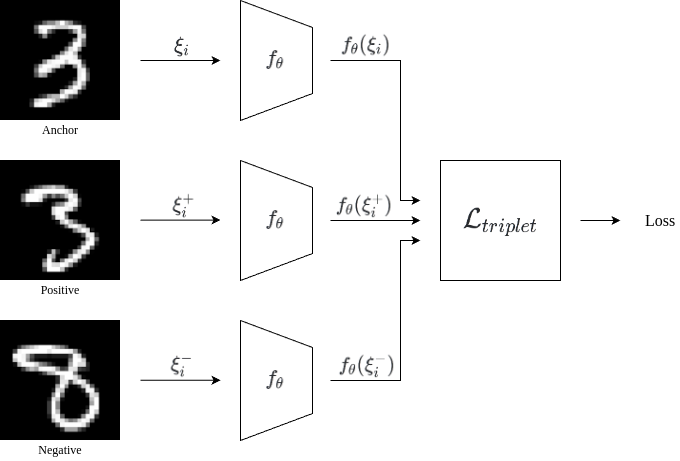
\includegraphics[width=0.75\textwidth]{figures/triplet_loss.png}
    \caption{Triplet Network structure for MNIST dataset \cite{lecun2010mnist}} \label{triplet-network:fig}
\end{figure}

In our research we employed a Convolutional Network architecture as $ f_{\theta} $ proposed by Lecun et al. \cite{Lecun_1998}. The detailed overview of the architecture, how to train it using Backpropagation algorithm, and their accuracy evaluation are out of scope for this paper, papers \cite{Beohar_2021,Krizhevsky_2012,Lecun_1998} have an extensive coverage of these topics.

When it comes to the sampling strategies of triplets $ (\xi_i, \xi^+_i, \xi^-_i) $, i.e., triplet mining, it's important to choose strategy that produces the most useful gradients for the objective function (\ref{triplet-loss-func:eq}). Xuan et al. \cite{xuan2020} discusses various strategies of online triplet mining, which selects triplets within each batch of a training set on each iteration. We employed the strategy of semi-hard triplet mining, where it chooses a anchor-negative pair that is farther than the anchor-positive pair, but within the margin $ \alpha $:

\begin{equation}
    \label{semi-hard-triplet-mining:eq}
    \xi^-_i = \argmin_{\substack{\xi: C(\xi_i) \neq C(\xi) \\ d(f_{\theta}(\xi_i), f_{\theta}(\xi)) > d(f_{\theta}(\xi_i), f_{\theta}(\xi^+_i))}} d(f_{\theta}(\xi_i), f_{\theta}(\xi))
\end{equation}

\noindent where $ C(\xi) $ - a label of an element $ \xi $.

By applying similar idea from \cite{Hoffer_2015,MURASAKI_ANDO_SHIMAMURA_2022,Turpault_Serizel_Vincent_2019}, we can use encoded latent representations of Triplet Network to train a Stochastic Quantization (\ref{sq-objective-fn-gradient:eq}) algorithm. This new approach allows is to solve supervised or semi-supervised learning problems of classification on high-dimensional data. Here is a breakdown of semi-supervised learning using combined algorithm, assuming we have labeled ratio $ \xi \subset \Xi $ and remaining unlabeled data $ \bar{\xi} \subset \Xi, \bar{\xi} \cap \xi = \varnothing $:

\begin{enumerate}
    \item train a Triplet Network $ f_{\theta} $ on labeled data $ \xi $ and produce encoded latent representations space $ \bar{\Xi} \subset \mathbb{R}^n $;
    \item use a Triplet Network $ f_{\theta} $ to project the remaining unlabeled data $ \bar{\xi} $ on the same latent representations space $ \bar{\Xi} $;
    \item use both labeled and unlabeled latent representations to train a Stochastic Quantization (\ref{sq-objective-fn-gradient:eq}) algorithm.
\end{enumerate}
